%% LyX 2.0.5.1 created this file.  For more info, see http://www.lyx.org/.
%% Do not edit unless you really know what you are doing.
\documentclass[usenatbib]{article}
\usepackage[latin9]{inputenc}
\usepackage[a4paper]{geometry}
\geometry{verbose}
\usepackage{color}
\usepackage{float}
\usepackage{graphicx}

\makeatletter

%%%%%%%%%%%%%%%%%%%%%%%%%%%%%% LyX specific LaTeX commands.
%% A simple dot to overcome graphicx limitations
\newcommand{\lyxdot}{.}


%%%%%%%%%%%%%%%%%%%%%%%%%%%%%% Textclass specific LaTeX commands.
\usepackage{jcappub}

%%%%%%%%%%%%%%%%%%%%%%%%%%%%%% User specified LaTeX commands.






%%%%%%%%%%%%%%%%%%%%%%%%%%%%%% LyX specific LaTeX commands.
%% A simple dot to overcome graphicx limitations
%Make my life significantly easier
\global\long\def\bd{{\bm{\delta}}}

\makeatother

\begin{document}

\title{The Maximum Circular Velocity Dependence of Halo Clustering}

\maketitle

\section{Introduction}

The halo model has been remarkably successful in describing observations
of galaxy clustering at many scales and many redshifts (give some
examples here). fundamental assumption clustering only depends on
the halo mass; not true because of assembly bias on large scales but
also ideas of eg. backsplashed halos. recent trend has been to populate
galaxies according to their maximum circular velocity. Describe why
this might be motivated \textemdash{} depends only on the central
part of the potential, set early in the growth of the halo (point
to Frank\textquoteright{}s recent paper here as an example). Also
may be more robust to disruption in mergers.

goal here is to discuss the dependence of galaxy clustering on the
central velocity dispersion both on small and large scales. We show
that some of the features in a detailed halo model come from the effects
of back-splash halos.


\section{The Simulation}

We use cosmological N-body simulations called the Bolshoi simulation
and the MultiDark simulation, described in XXX and XXX respectively,
to investigate the maximum circular velocity dependence of halo clustering.
The Bolshoi simulation uses $2048^{3}$ particles with a volume of
$(250$$h^{-1}{\rm Mpc})^{3}$, while the MultiDark simulation uses
the same number of particles as the Bolshoi simulation but with a
volume of ($1h^{-1}{\rm Gpc})^{3}$. Both simulations assumes a flat
$\Lambda{\rm CDM}$ model with density parameters $\Omega_{m}=0.27$,
$\Omega_{\Lambda}=0.73$, $\Omega_{b}=0.0469$, and $\sigma_{8}=0.82$,
$n=0.95$, $h=0.70$. (??Do I need to put a name for each constant?)The
details of the simulations are described in XXX. For halo identification,
we use the ROCKSTAR halo finder (XXX) where the halo masses and maximum
circular velocities are computed from bound particles. 

??Should I explain more about what bound particles mean (though my
understanding is vague...) and am not so sure what other ways to define
masses and circular velocity and also how the definitions can make
things different...

??What other information do I need to put here?


\section{The Maximum Circular Velocity Dependence of Halo Clustering}

In this section, we investigate the maximum circular velocity dependence
of halo clustering on both large and small scales. In order to do
that, we compute correlation functions and measure halo biases for
halo samples having different maximum circular velocities. We first
describe how we select halos for each sample and then show how those
samples have different clustering properties.


\subsection{The Maximum Circular Velocity}

As shown in Fig. \ref{fig:vmax-mvir}, the maximum circular velocity
and halo mass has tight correlation, and yet the scatter between the
maximum circular velocity and halo mass becomes larger with decreasing
halo masses. In fact, we can compute an expected maximum circular
velocity from halo mass

\begin{equation}
\overline{V}_{{\rm max}}=0.465M_{{\rm vir}}^{1/3}\sqrt{G(\frac{4}{3}\pi\Delta_{{\rm h}}\rho_{{\rm crit}}\Omega_{m})^{1/3}\frac{c}{{\rm ln(1+c)-c/(1+c)}}},\label{eq:vmax-mvir}
\end{equation}
where $V_{{\rm max}}$ is the maximum circular velocity and $M_{{\rm vir}}$
is the halo mass, $\Delta_{{\rm h}}$ is the overdensity limit which
defines the virial radius, and $c$ is the concentration parameter.
Eq. \ref{eq:vmax-mvir} comes from an NFW profile (\textcolor{red}{citation}).
To obtain Eq. \ref{eq:vmax-mvir}, we use the concentration of 
\begin{equation}
{\rm log}_{10}c=-0.097{\rm log_{10}M_{vir}}+2.148.
\end{equation}
(??Ask Frank how he obtain this concentration value and why this is
a reasonable value) \textcolor{black}{In Fig. \ref{fig:vmax-mvir},
this $V_{{\rm max}}-M_{{\rm vir}}$ relation with the above concentration
(shown as a red solid line) intersects the peak of the distribution,
which means that many of the halos follow this relation.}


\subsection{Samples}

\begin{figure}
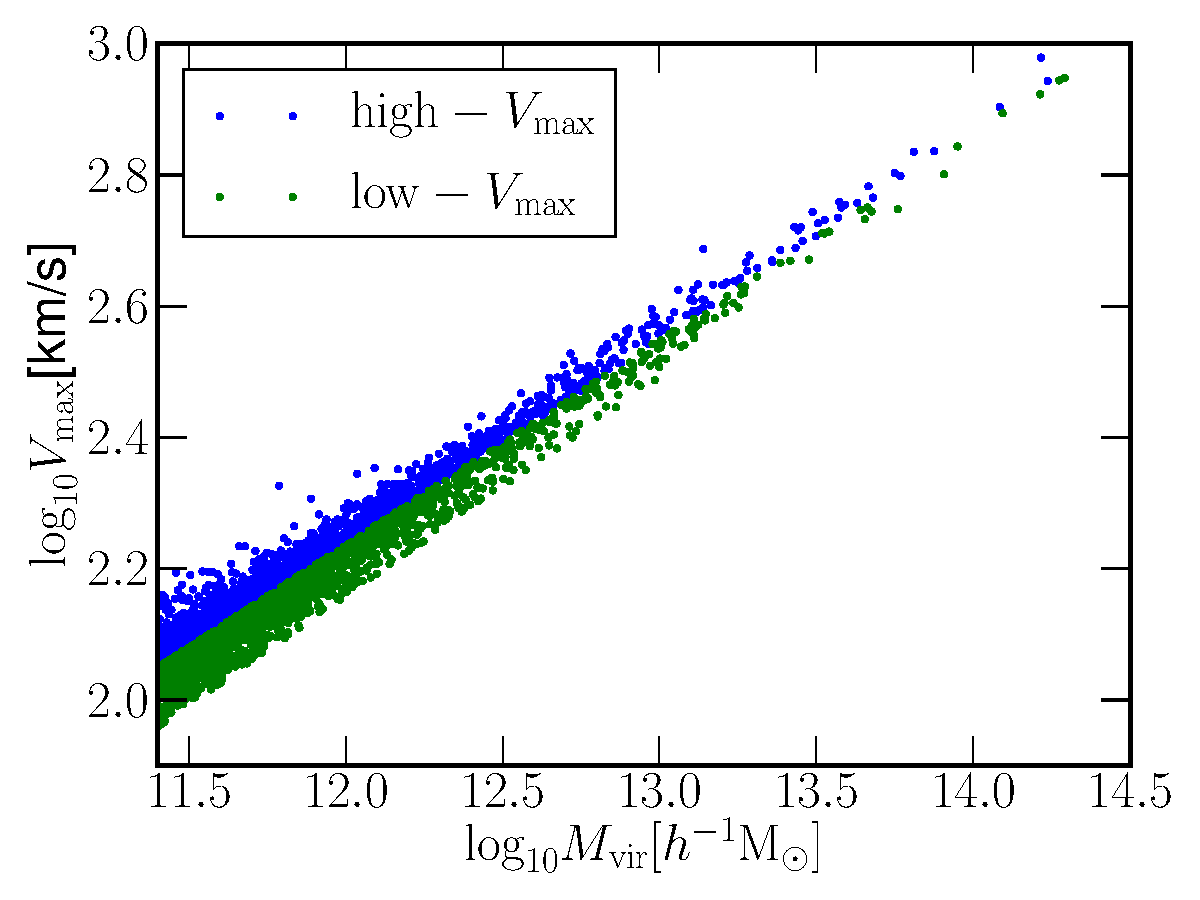
\includegraphics[width=0.5\columnwidth]{/Users/old_ts485/Desktop/biasVmax/plots/logVmax_logMvir_Dh360}

\caption{\label{fig:vmax-mvir}Distribution of halo mass and the maximum circular
velocity at $z=0.0$ for halos whose masses are between $10^{12.5}{\rm M_{\odot}}$
and $10^{13.0}{\rm M_{\odot}}$. The blue dots represent halos whose
maximum circular velocity is greater than $\overline{V}_{mas}$, while
the green dots are the ones with smaller $V_{max,obs}$ than $\overline{V}_{max}$.
The boundary between blue and green dots corrspond to $\overline{V}_{max}$
computed from Eq. \ref{eq:vmax-mvir}.}
\end{figure}


The above equation is a one to one mapping between the virial mass
of the halo and its maximum circular velocity. Given this mapping,
we can translate clustering measurements as a function of halo mass
into predicted clustering measurements as a function of maximum circular
velocity. Our goal below is to determine whether this conversion describes
the measured clustering or if there is a residual dependence on the
maximum circular velocity. In order to explore this, we first split
the sample into a sequence of virial mass bins, chosen such that there
are the same numbers of halos in each bin. This process is reminiscent
of an abundance-matching procedure (cite XXX). We then further split
each bin into two subsamples with their observed $V_{{\rm max,obs}}$
greater than (denoted by ``upper'') or less than (denoted as ``lower'')
$V_{{\rm max}}(M_{{\rm vir}})$. This selection ensures that both
the upper and lower subsamples have the same mean halo mass. Therefore,
in the absence of an additional $M_{vir}$ dependence (??isn't this
$M_{{\rm vir}}$ dependence?) on clustering, these samples should
have the same clustering properties. Note that this would not be true
if we had simply split the sample along $V_{{\rm max}}$, since the
two resulting subsamples would have different mean halo masses. 


\subsection{Mvir-based samples}

In order to measure halo biases, we compute halo-matter cross correlation
functions for each subsample and measure a linear bias 
\begin{equation}
b_{lin}=<\xi_{hm}(r)/\xi_{mm}(r)>,
\end{equation}
where $\xi_{hm}$ and $\xi_{mm}$ are halo-matter and matter-matter
correlation functions and we take the average of the ratio on $r$
from $10h^{-1}{\rm Mpc}$ to $20h^{-1}{\rm Mpc}$ (??may change to
jackknife samplings). Here, instead of using full DM particles, we
subsample $1000000$ particles to compute matter auto correlation
functions. The reason we use cross correlation functions is to reduce
the shot noise effect on the error.

In Fig. \ref{fig:linear-bias}, we show how linear biases depend on
the maximum circular velocity as a function of halo mass. We compute
linear biases for each mass bin classifying into ``upper'' and ``lower''
maximum circular velocity halos. The halos which have different maximum
circular velocity clearly cluster differently. Furthermore, the relative
bias of ``upper'' versus ``lower'' subsamples increases with decreasing
halo mass to almost 40\% on low mass end.

\begin{figure}
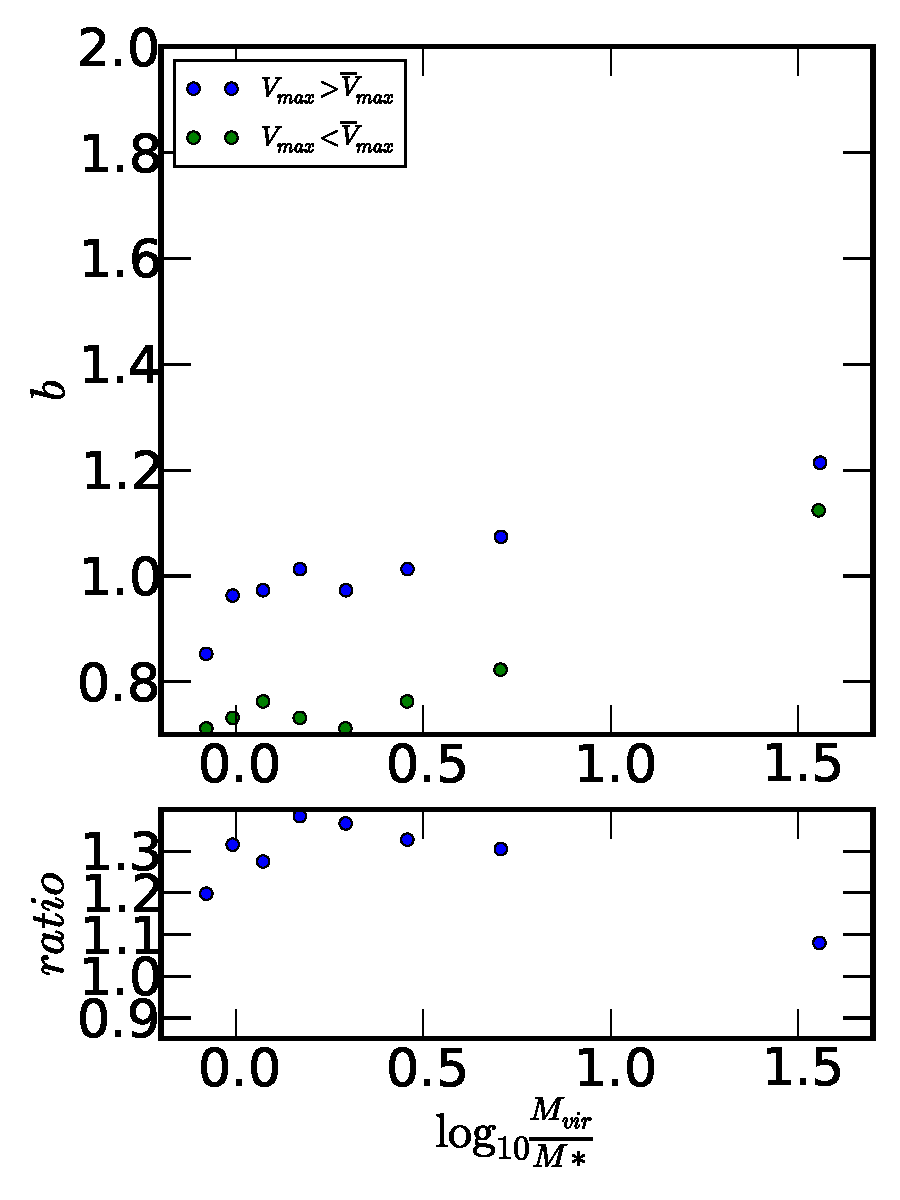
\includegraphics[width=0.5\columnwidth]{/Users/old_ts485/Desktop/biasVmax/plots/linearBias_wang_Bolshoi}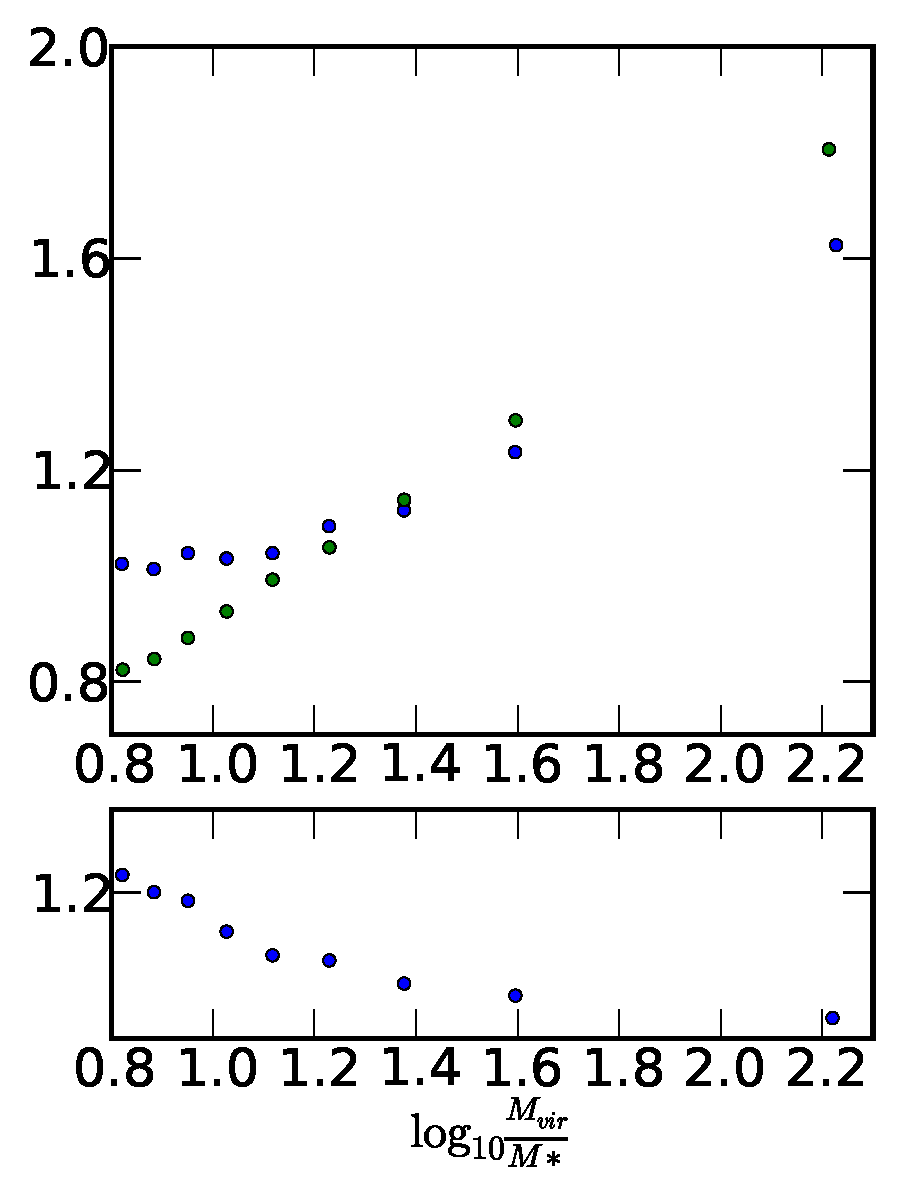
\includegraphics[width=0.5\columnwidth]{/Users/old_ts485/Desktop/biasVmax/plots/linearBias_wang_MultiDark}

\caption{\label{fig:linear-bias}Upper panel: Linear bias at $z=0.0$ as a
function of halo mass from the Bolshoi simulation (left) and the MultiDark
simulation (right). The blue circles represents a linear bias for
halos whose maximum circular velocities are greater than $\overline{V}_{max}$,
while the green circles correspond to halos whose maximum circular
velocities are smaller than $\overline{V}_{max}$. Lower panel: Ratio
of linear biases between ``upper'' (i.e., $V_{max,obs}>\overline{V}_{max}$)
and ``lower'' (i.e., $V_{max,obs}<\overline{V}_{max}$) samples
from the Bolshoi simulation (left) and the MultiDark simulation (right).
As halo masses decrease, the difference on linear bias between ``upper''
and ``lower'' subsamples becomes larger up to 40\%. Here, $M*=10^{11.5}{\rm M_{\odot}}$.}
\end{figure}


In Fig. \ref{fig:small-scale}, we investigate the maximum circular
velocity dependence of halo bias on small scales. On small scales,
a halo bias is scale-dependent. The question here is whether halos
with different maximum circular velocity have different scale-dependence
on their biases. In order to find that, we take the ratio of halo-matter
cross correlation functions between ``upper'' and ``lower'' subsamples
and normalize it by their linear biases. Fig. \ref{fig:small-scale}
clearly shows that the scale-dependence depends on the maximum circular
velocity and its Vmax-dependence is mass-dependent. As halo mass decreases,
the relative scale-dependence between ``upper'' and ``lower''
subsamples increases, especially halos with large maximum circular
velocities heavily clustered around $1h^{-1}{\rm Mpc}$.

\begin{figure}[H]
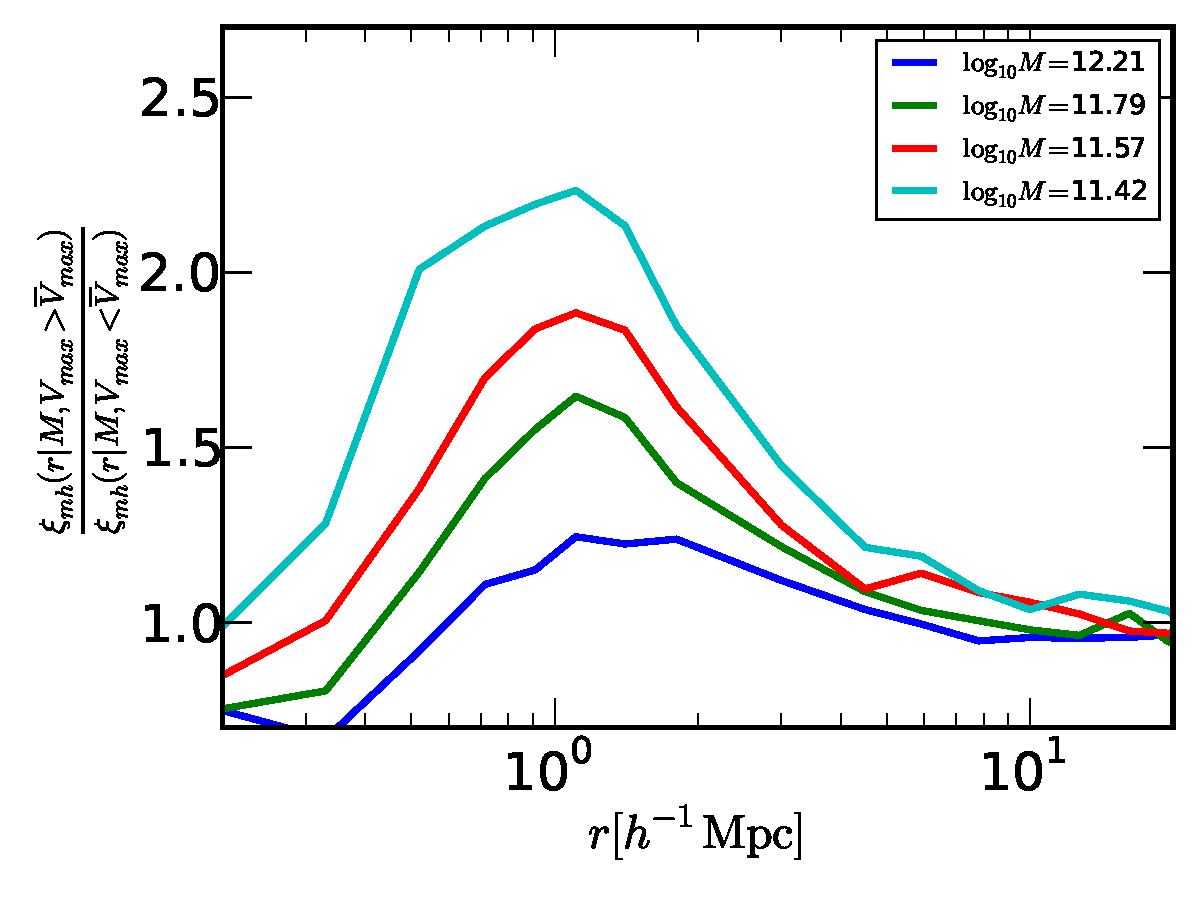
\includegraphics[width=0.5\columnwidth]{/Users/old_ts485/Desktop/biasVmax/plots/Bolshoi_smallScale_wang_log}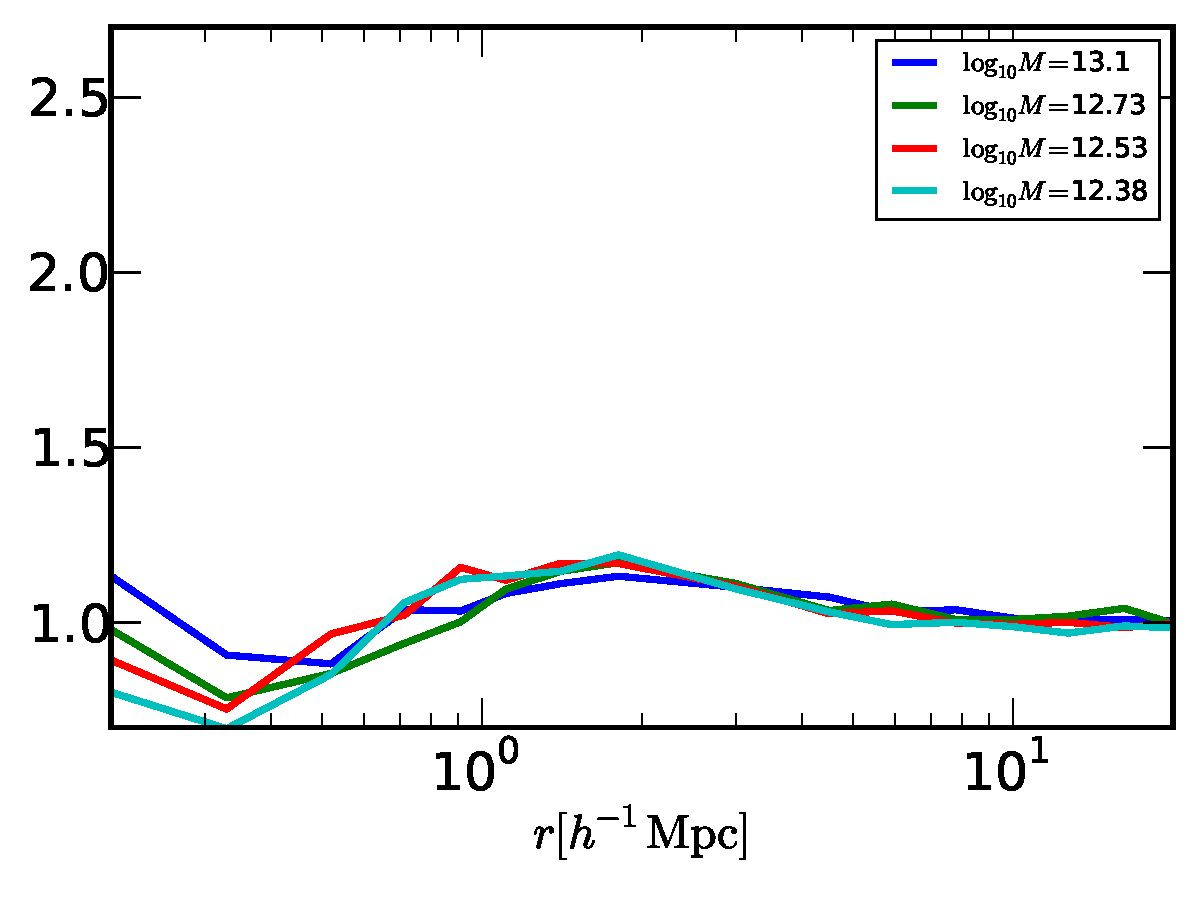
\includegraphics[width=0.5\columnwidth]{/Users/old_ts485/Desktop/biasVmax/plots/MultiDark_smallScale_wang_log}

\caption{\label{fig:small-scale}Ratio of halo-matter cross correlation functions
between ``upper'' and ``lower'' subsamples normalized by their
linear biases. The plots are from the Bolshoi simulation (left) and
the MultiDark simulation (right) at z = 0.0. Each line corresponds
to different halo mass bins labeled in the plots. Those plots show
that ``upper'' and ``lower'' subsamples have different scale-dependence
on small scales and the relative scale-dependence between those subsamples
increases smoothly with decreasing halo mass. }


\end{figure}


\begin{figure}[H]
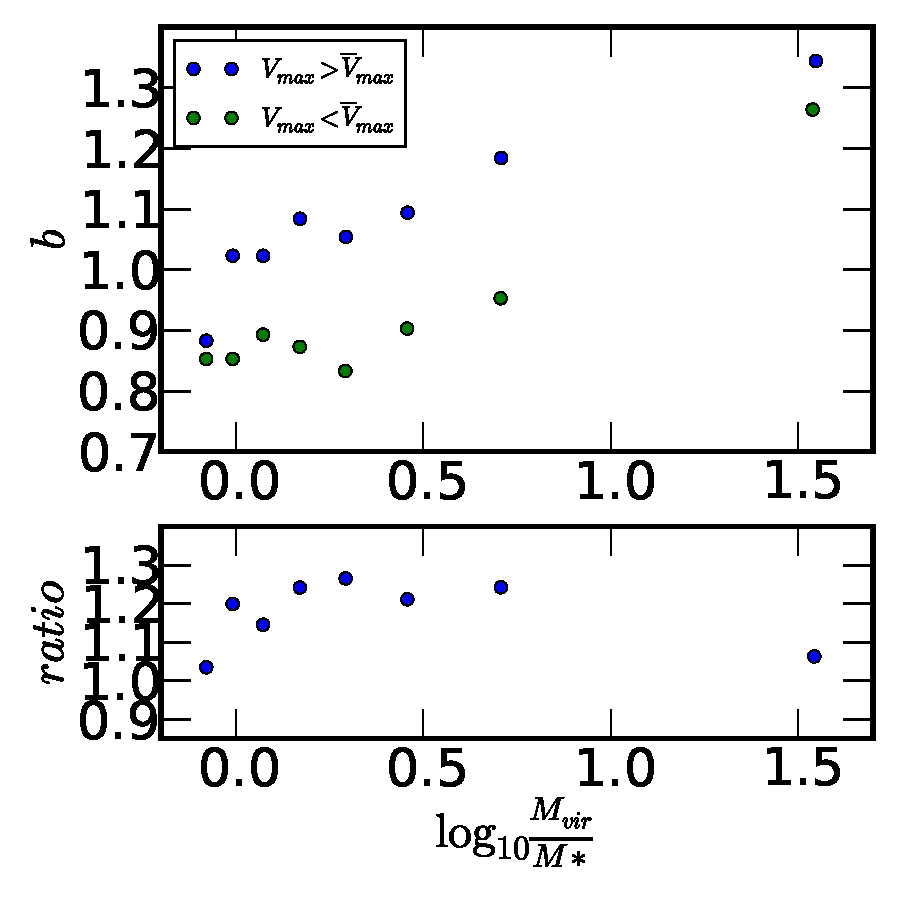
\includegraphics[height=0.5\columnwidth]{/Users/old_ts485/Desktop/biasVmax/plots/linearBias_wang_Bolshoi_eje}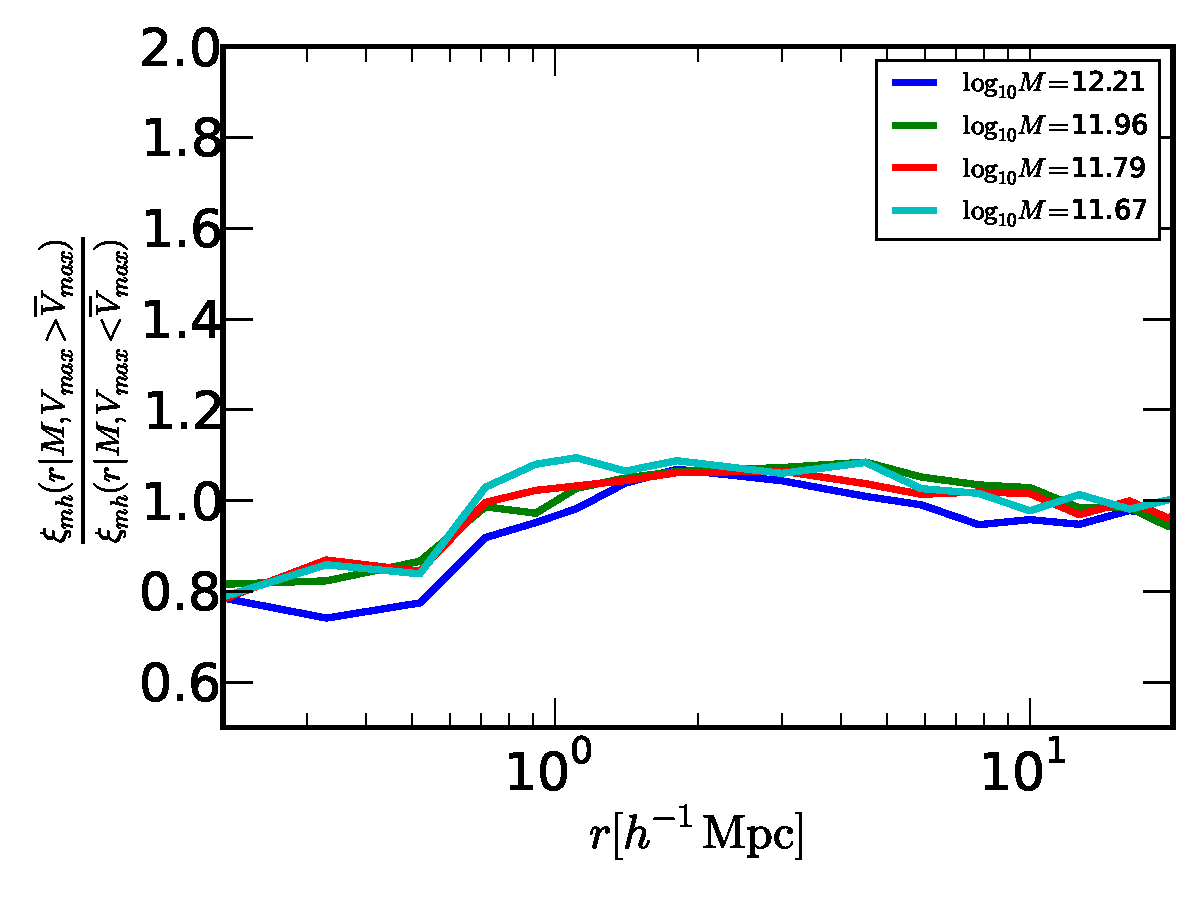
\includegraphics[width=0.5\columnwidth]{/Users/old_ts485/Desktop/biasVmax/plots/Bolshoi_smallScale_nonEj_wang_log}

\caption{The same figures as Fig. \ref{fig:linear-bias} (left) and Fig. \ref{fig:small-scale}
(right) without ejected halos. We use halos from the Bolshoi simulation
at $z=0.0$, because we could not find many ejected halos in the MultiDark
simulation due to its mass resolution. The left panel shows the linear
bias as a function of halo mass for the halos whose $V_{max}$ greater/less
than $\bar{V}_{max}$ and their ratio between those subsamples. The
difference in linear biases without ejected halos is suppressed on
small halos close to $M^{*}$, while there is little difference between
the ratio with and without ejected halos on large mass end. The right
panel shows the ratio of halo-matter cross correlation functions between
``upper'' and ``lower'' subsamples normallized by their linear
biases. It is obvious that the scale-dependent clustering difference
is now mostly removed by excluding ejected halos from samples. }


\end{figure}


{*}need some explanations for the decrease of the relative bias on
the lowest mass end? is it real or artificial?

{*}use jackknife sampling to put error bars


\section{Applications}


\subsection{Mvir-based v.s. Vmax-based}

\begin{figure}[H]
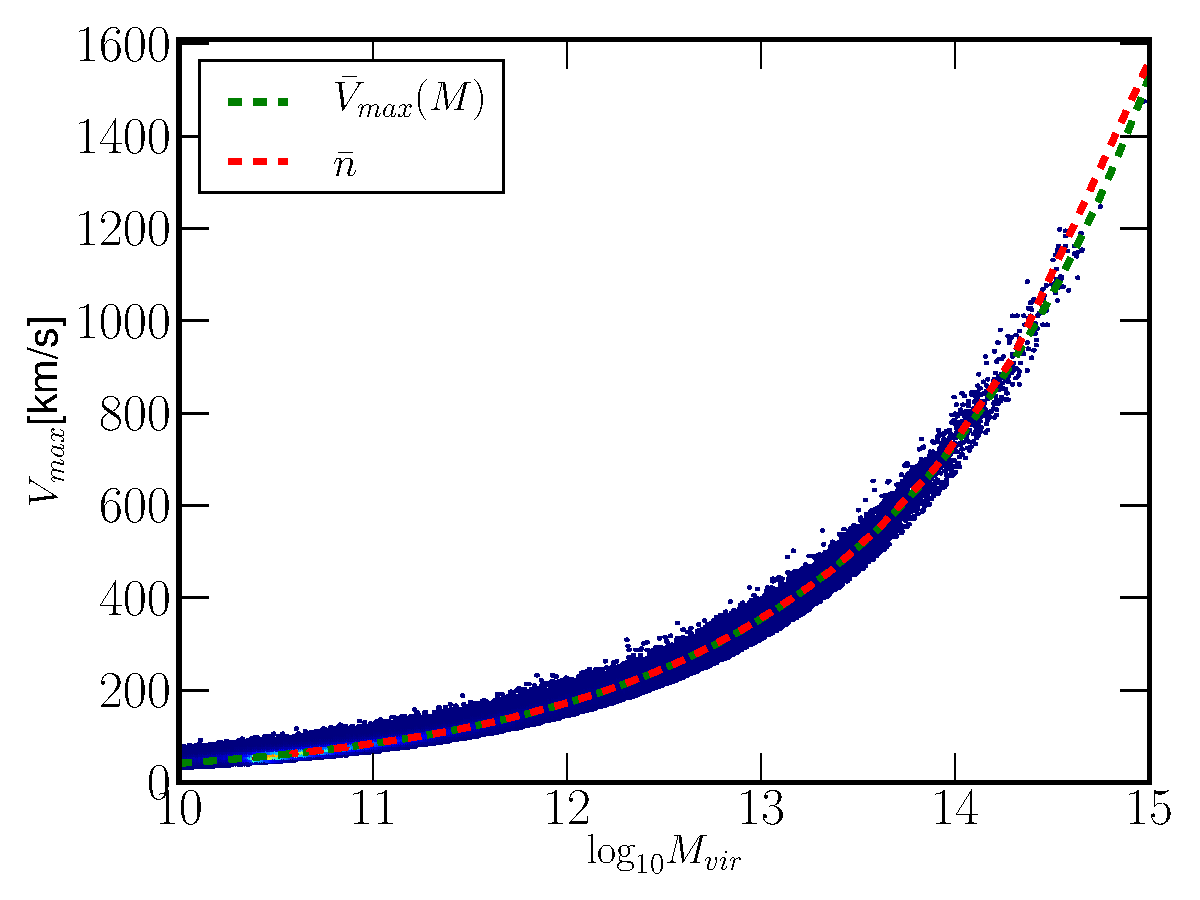
\includegraphics[width=0.5\columnwidth]{/Users/old_ts485/Desktop/biasVmax/plots/logMhalo_Vcir_nbar_Bolshoi}

\caption{\label{fig:nbar}Distribution of halo mass and the maximum circular
velocity as a countour plot, overplotted $\overline{V}_{max}$ (as
a green dashed line) and the correspondence between $M_{vir}$ and
$V_{max}$ in abundance matching (as a red dashed line labeled as
$\overline{n}$). The plot shows that $\overline{V}_{max}$ and the
correspondence in abundance matching overlaps on most of halo mass
scales.}


\end{figure}


\begin{figure}[H]
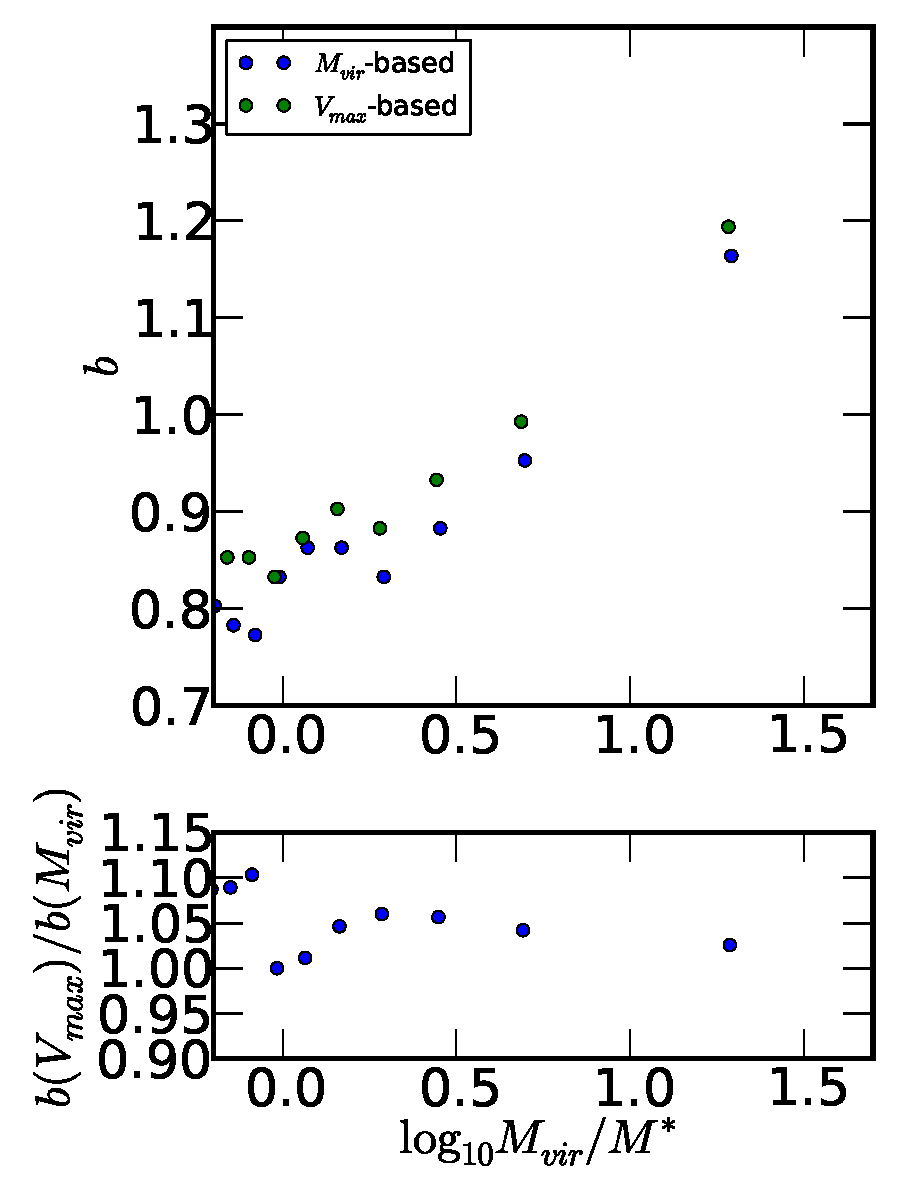
\includegraphics[height=0.5\columnwidth]{/Users/old_ts485/Desktop/biasVmax/plots/linearBias_andrew_Bolshoi}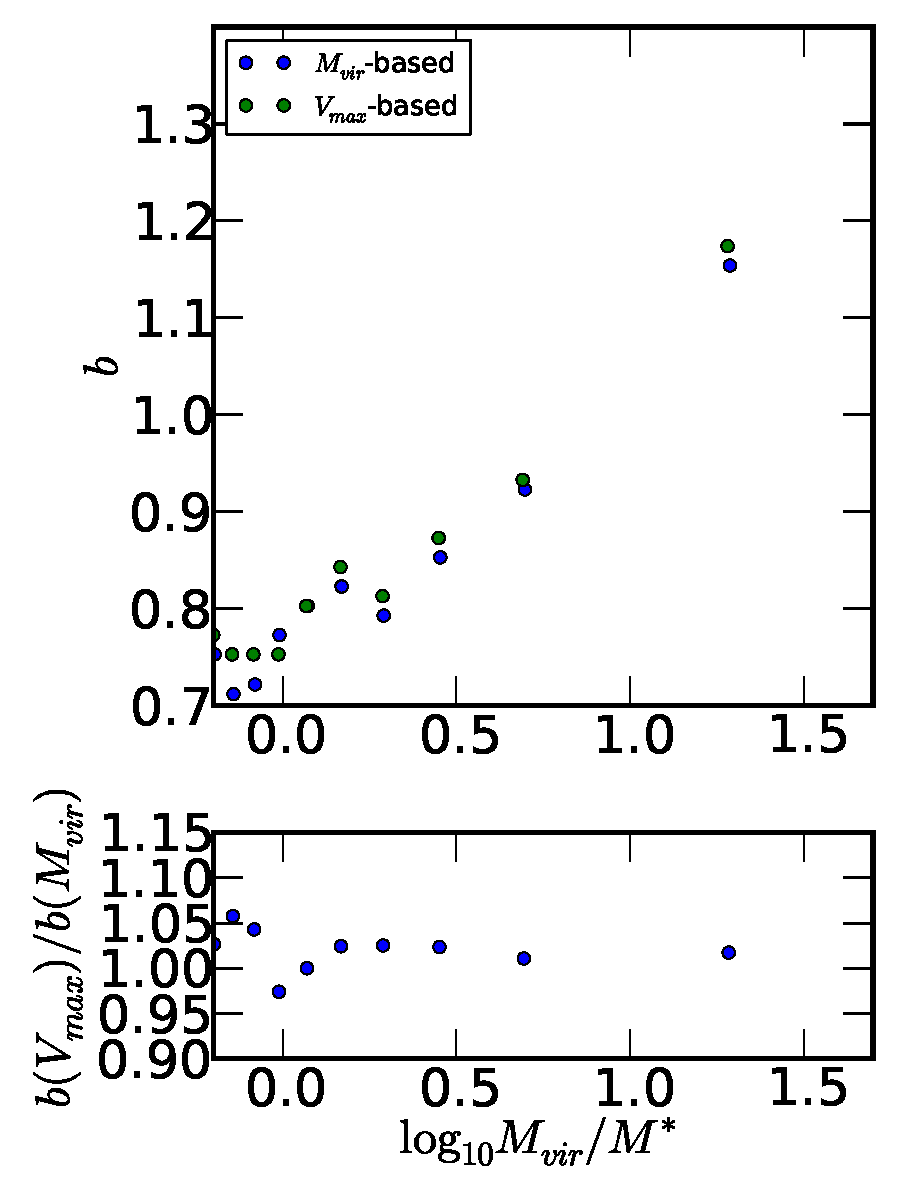
\includegraphics[height=0.5\columnwidth]{/Users/old_ts485/Desktop/biasVmax/plots/linearBias_andrew_Bolshoi_nonEj}\caption{\label{fig:abundance_linear}Upper panel: We compare linear biases
for halos selected by abundance matching for halo mass (blue dots)
and the maximum circular velocity (green dots) as a function of halo
mass where $M^{*}=10^{11.5}{\rm M_{\odot}}$. As shown in Fig. \ref{fig:nbar},
we can find a corresponding $V_{max}$ for those samples through Eq.
\ref{eq:vmax-mvir}. The left panel is the result including ejected
halos, while the right panel is the one without ejected halos. The
linear biases overall decrease by excluding ejected halos for both
$M_{vir}$-based and $V_{max}$-based abundance matching samples.
Lower panel: Ratio of linear biases between $M_{vir}$-based and $V_{max}$-based
abundance matching samples with ejected halos (left) and without ejected
halos (right). The difference between those samples become smaller
by at most factor of 2.}


\end{figure}


\begin{figure}[H]
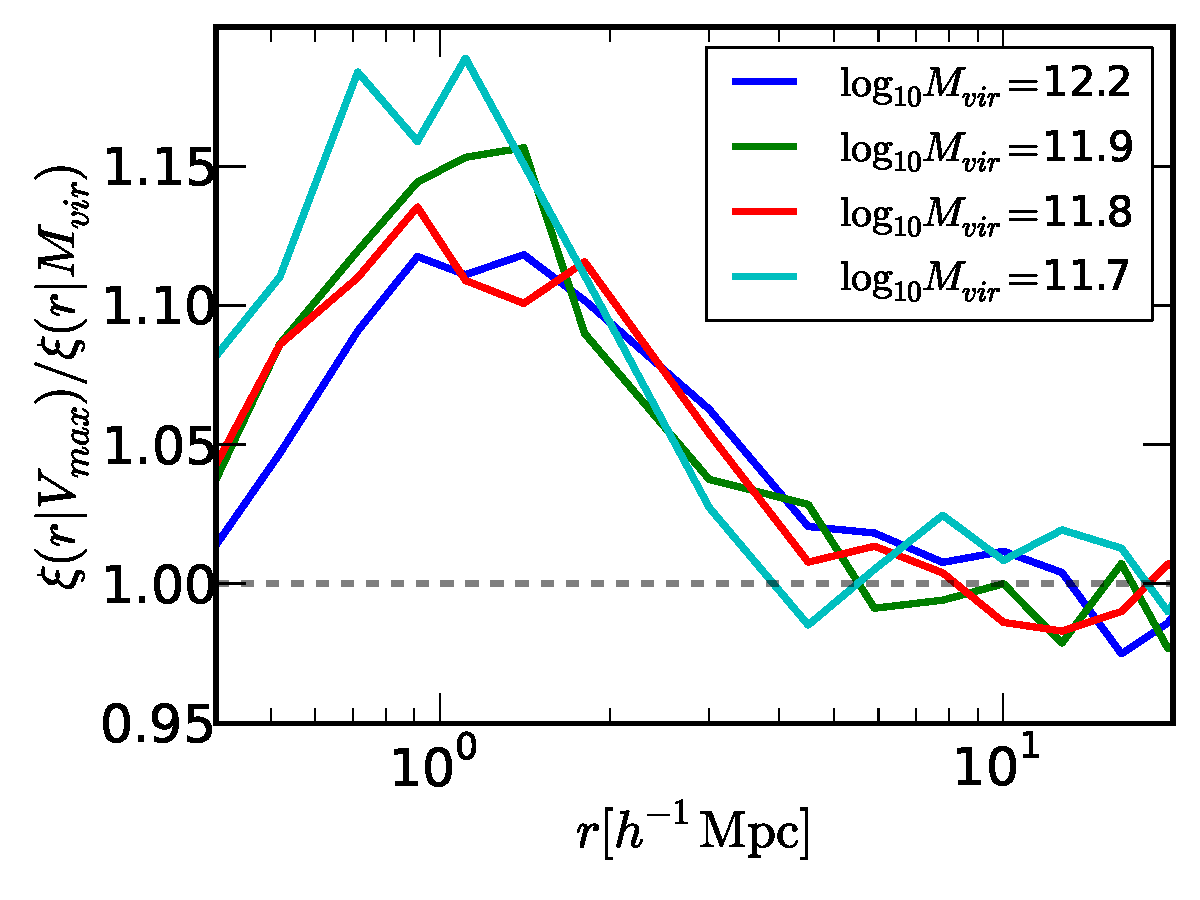
\includegraphics[width=0.5\columnwidth]{/Users/old_ts485/Desktop/biasVmax/plots/Bolshoi_andrew_smallScale}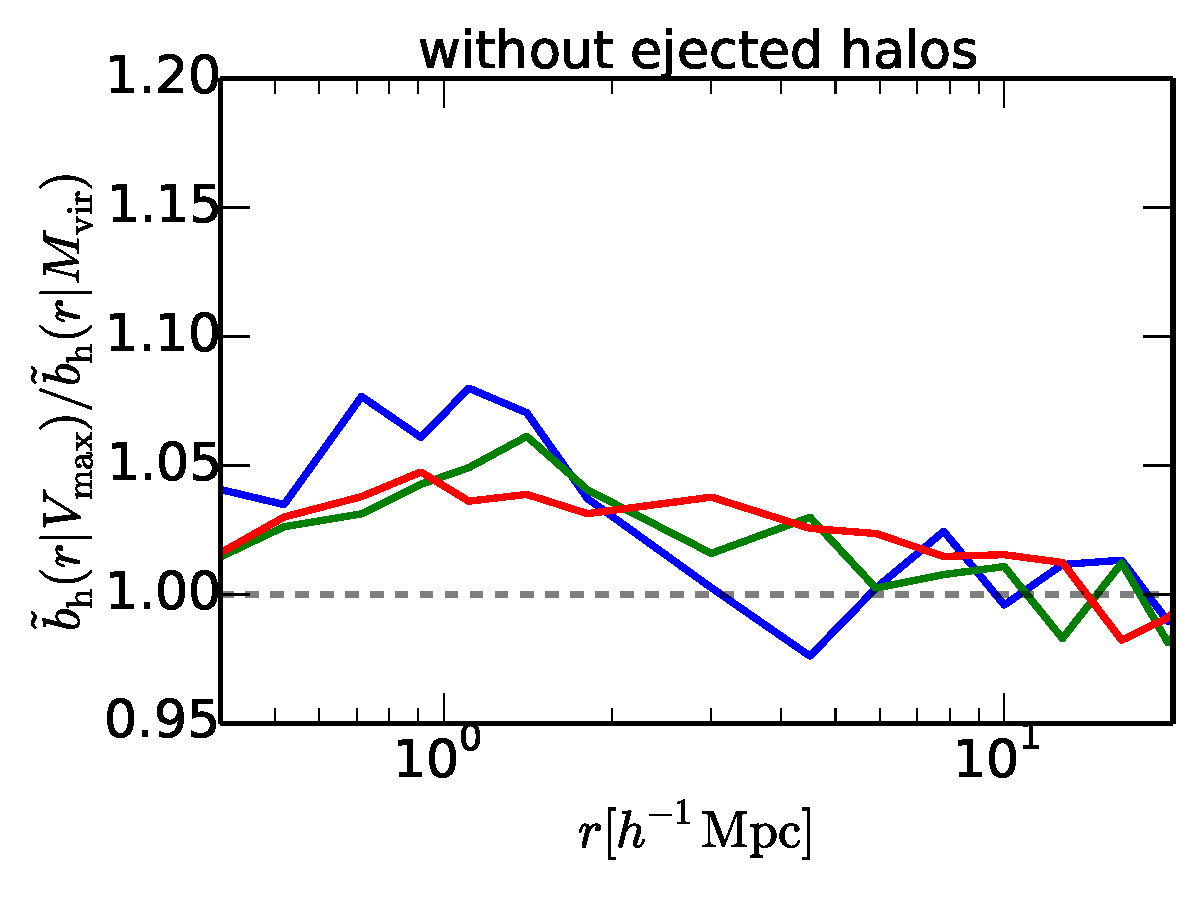
\includegraphics[width=0.5\columnwidth]{/Users/old_ts485/Desktop/biasVmax/plots/Bolshoi_andrew_smallScale_nonEj}

\caption{\label{fig:abundance_small}Ratio of halo-matter cross correlation
functions between$M_{vir}$-based and $V_{max}$-based abundance matching
samples with ejected halos (left) and without ejected halos (right).
The ratios are normalized by their linear biases. Each line corresponds
to different halo mass bins labeled in the plots (which can be translated
into corresponding $\overline{V}_{max}$ through Eq. \ref{eq:vmax-mvir}).
When samples contain ejected halos, there is a strong scale-dependent
difference between those two different abundance matching samples
around $1h^{-1}{\rm Mpc}$. By excluding ejected halos, the difference
is more or less removed.}


\end{figure}



\subsection{$\Delta\Sigma(r)$}


\subsection{MergerTree's Vmax v.s. Vmax,obs}


\section{Discussion}

(Option)
\begin{figure}[H]
\includegraphics[width=0.5\columnwidth]{/Users/old_ts485/Downloads/dist2_nearestCluster_m11\lyxdot 7to11\lyxdot 8}

\caption{Histogram of distances to the nearest Clusters (defined as $M_{vir}>10^{14}{\rm M_{\odot}}$)
for non-ejected halos and ejected halos: Right now, I only have the
one for all the halos...may change to the plot of fractions: Is it
reasonable to play with the cluster masses? Also, make the similar
plots for nearest massive halos by separating ejected and non-ejected
halos (upper/lower)...}
\end{figure}

\end{document}
